\chapter{Basics}

\section{Fundamental Theorem of Linear Algebra}

\begin{center}
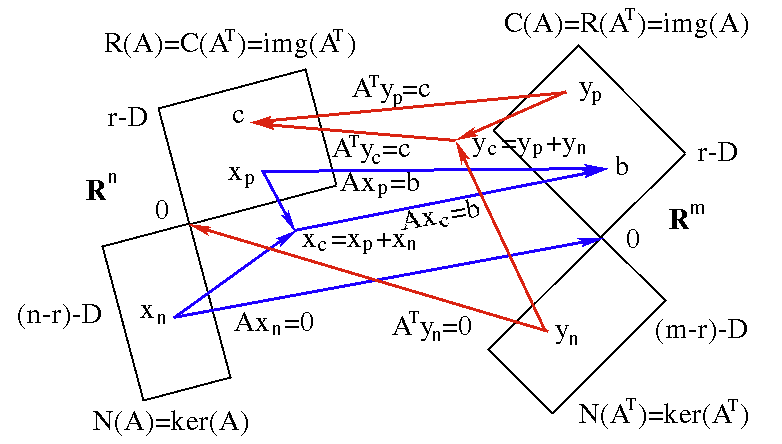
\includegraphics[width=\textwidth]{imgs/fund_theorem_lin_alg1.png}
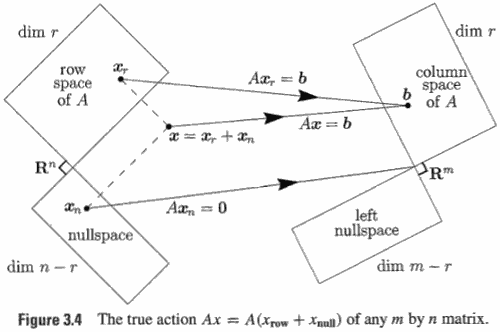
\includegraphics[width=\textwidth]{imgs/fund_theorem_lin_alg2.png}
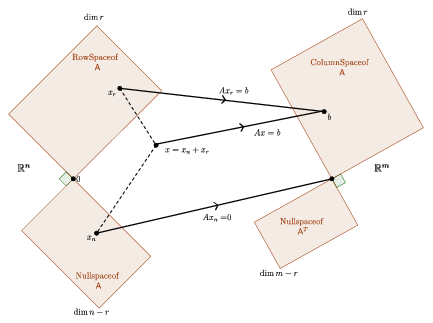
\includegraphics[width=\textwidth]{imgs/fund_theorem_lin_alg3.png}
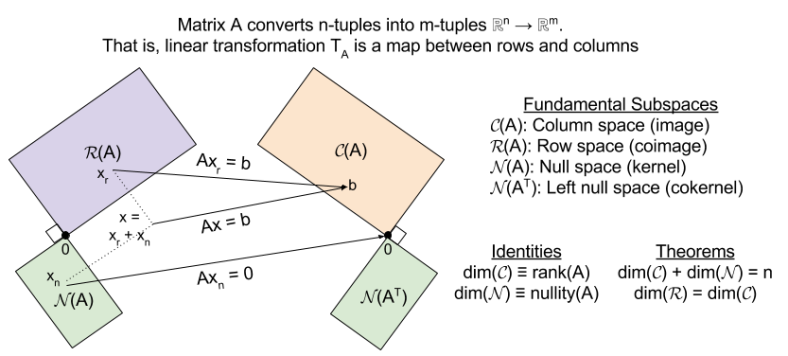
\includegraphics[width=\textwidth]{imgs/fund_theorem_lin_alg4.png}
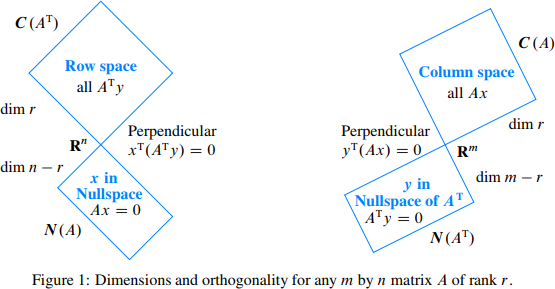
\includegraphics[width=\textwidth]{imgs/fund_theorem_lin_alg5.png}
\end{center}


\section{Matrix Properties}

\begin{align}
\mA(\mB+\mC) &=   \mA\mB+\mA\mC &\textrm{(left distributivity)}   \\
(\mB+\mC)\mA &=   \mB\mA+\mC\mA &\textrm{(right distributivity)}  \\
\mA\mB       &\ne \mB\mA        &\textrm{(in general)}            \\
(\mA\mB)\mC  &=   \mA(\mB\mC)   &\textrm{(associativity)}
\end{align}

\section{Rank}

\begin{align}
\noalign{If $\mA\in\sRmn$ and $\mB\in\sRnr$, then}
\eqcite{Thome2016}
\rank(\mA)+\rank(\mB)-n\le \rank(\mA\mB)\le \min(\rank(\mA),\rank(\mB)) &&~~~~\textrm{Sylvester's Inequality} \\
\noalign{If $\mA\mB$, $\mA\mB\mC$, $\mB\mC$ are defined, then}
\eqcite{Thome2016}
\rank(\mA\mB)+\rank(\mB\mC)\le \rank(\mB)+\rank(\mA\mB\mC) && \textrm{Frobenius's inequality} \\
\noalign{If $\dim(\mA)=\dim(\mB)$, then}
\rank(\mA+\mB)\le\rank(\mA)+\rank(\mB) &&\textrm{Subadditivity}
\end{align}
If $\mA_1, \mA_2, \ldots, \mA_l$ have $n_1,n_2,\ldots,n_l$ columns, so that $\mA_1\mA_2\ldots\mA_l$ is well-defined, then
\begin{equation}
\eqcite{Thome2016}
\rank(\mA_1\mA_2\ldots\mA_l)
\ge \sum_{i=1}^{l-1}\rank(\mA_i\mA_{i+1})-\sum_{i=2}^{l-1}\rank(\mA_i)
\ge\sum_{i=1}^l\rank(\mA_i)-\sum_{i=1}^{l-1}n_i
\end{equation}

\section{Identities}
\begin{align}
\left(\sum_{i=1}^n \vz_i\right)^2 = \vz^T
\begin{bmatrix}
1      & \hdots & 1      \\
\vdots & \ddots & \vdots \\
1      & \hdots & 1
\end{bmatrix}
\vz
\end{align}

\section{Matrix Multiplication}

For $\mA\in\sR^{i,j}$ and $\mB\in\sR^{j,k}$ and $\mC\in\sR^{l,k}$
\begin{align}
[\mA\mB]_{ik} &= \sum_j \mA_{ij}\mB_{jk} \\
[\mA\mB\mC^T]_{il} &= \sum_j \mA_{ij}[\mB\mC^T]_{jl}=\sum_j \mA_{ij}\sum_k \mB_{jk}\mC_{lk}=\sum_j\sum_k \mA_{ij}\mB_{jk}\mC_{lk}
\end{align}
%TODO: Algorithms and orderings



\section{Transpose Properties}

\begin{align}
(c\mA)^T            &= c\mA^T                \\
(\mA\mB)^T          &= \mB^T\mA^T            \\
(\mA\mB\mC\ldots)^T &= \ldots\mC^T\mB^T\mA^T \\
(\mA+\mB)^T         &= \mA^T+\mB^T           \\
(\mA+\mB+\ldots)^T  &= \mA^T+\mB^T+\ldots^T  \\
(\mA^{-1})^T        &= (\mA^T)^{-1}
\end{align}

\section{Conjugate Tranpose}

\begin{align}
(\mA^H)^{-1}        &= (\mA^{-1})^H          \\
(\mA+\mB)^H         &= \mA^H+\mB^H           \\
(\mA+\mB+\ldots)^H  &= \mA^H+\mB^H+\ldots^H  \\
(\mA\mB)^H          &= \mB^H \mA^H           \\
(\mA\mB\mC\ldots)^H &= \ldots\mC^H\mB^H\mA^H
\end{align}


\section{Determinant Properties}
The determinant is only defined for square matrices; here we assume that $\mA\in\sRnn$.

\begin{align}
\det(\mI_n)        &= 1                                   \\
\det(\mA^T)        &= \det(\mA)                           \\
\det(\mA^H)        &= \det(\mA)^H                         \\
\det(\mA^{-1})     &= 1/\det(\mA)                         \\
\det(\mA\mB)       &= \det(\mB\mA)                        \\
\det(\mA\mB)       &= \det(\mA)\det(\mB)                  &\mB\in\sRnn \\
\det(c\mA)         &= c^n\det(\mA)                        \\
\det(\mA)          &= \prod \eig(\mA)                     \\
\det(\mA^n)        &= \det(\mA)^n                         \\
\det(-\mA)         &= (-1)^n\det(\mA)                     \\
\det(\mA^c)        &= \det(\mA)^c                         \\
\det(\mI+\vu \vv^T)&= 1 + \vu^T \vv                       \\
\det(\mB\mA\mB^{-1}) &= \det(\mA)                         \\
\det(\mB\mA\mB^{-1}-c\mI) &= \det(\mA-c\mI)               \\
\noalign{For n=2:}
\det(\mI+\mA)      &= 1 + \det(\mA)+\trace(\mA) \\
\det(\mA) &=\begin{vmatrix} a & b \\ c & d \end{vmatrix} = ad-bc \\
\noalign{For n=3:}
\det(\mI+\mA)      &= 1 + \det(\mA)+\trace(\mA) + \frac{1}{2}\trace(\mA)^2-\frac{1}{2}\trace(\mA^2) \\
\det(\mA) &=\begin{vmatrix} a & b & c \\ d & e & f \\ g & h & i \end{vmatrix} =
 a\begin{vmatrix} e & f \\ h & i \end{vmatrix}
-b\begin{vmatrix} d & f \\ g & i \end{vmatrix}
+c\begin{vmatrix} d & e \\ g & h \end{vmatrix} \\
\noalign{For n=4:}
\det(\mI+\mA)      &= 1 + \det(\mA)+\trace(\mA) + \frac{1}{2}\trace(\mA)^2-\frac{1}{2}\trace(\mA^2)  \\
                   &    + \frac{1}{6}\trace(\mA)^3-\frac{1}{2}\trace(\mA)\trace(\mA^2)+\frac{1}{3}\trace(\mA^3) \\
\noalign{For small $\epsilon$:}
\det(\mI+\epsilon\mA) &\approx 1 + \det(\mA) + \epsilon\trace(\mA)+\frac{1}{2}\epsilon^2\trace(\mA)^2-\frac{1}{2}\epsilon^2\trace(\mA^2) \\ %TODO: Check from MatrixCookbook
\det(\mI+\epsilon\mA) &\approx 1 + \epsilon\trace(\mA) + O(\epsilon^2) \\ %TODO: Check: From MathWorld
\noalign{Sylvester's determinant identity, for $\mA\in\sRmn, \mB\in\sRnm$}
\eqcite{Sylvester1851}
\det(\mI_m+\mA\mB) &= \det(\mI_n+\mB\mA)                    \\
\det(\mX+\mA\mB)   &= \det(\mX)\det(\mI_n + \mB\mX^{-1}\mA) \\
\noalign{If $\mA$ is triangular}
\det(\mA) &= \prod_i \mA_{i,i} = \prod_i \diag(\mA)_i \\
\noalign{If all entries of $\mA\in\sCnn$ are in the unit disk}
\det(\mA)\le n^{n/2} \eqcite{Hadamard1893} \\
\noalign{Schur's determinant identities}
\det(\mM) &= \det(\begin{bmatrix} \mA & \mB \\ \mC & \mD \end{bmatrix}) = \det(\mA) \det(\mD -\mC \mA^{-1}\mB) \\
\det(\mM) &= \det(\begin{bmatrix} \mA & \mB \\ \mC & \mD \end{bmatrix}) = \det(\mD) \det(\mA -\mB \mD^{-1}\mC) \\
\end{align}
%TODO: Matix exponential identities det(A)=log(det(exp(A)))

Geometrically, if a unit volume is acted on by $\mA$, then $|\det(\mA)|$ indicates the volume after the transformation.


\section{Trace Properties}
The Trace is only defined for square matrices.
\begin{align}
\trace(\mA)      &=\sum_i \mA_{ii}               \\
\trace(\mA)      &=\sum_i \eig(\mA)              \\
\trace(\mA+\mB)  &=\trace(\mA)+\trace(\mB)       \\
\trace(c\mA)     &=c\trace(\mA)                  \\
\trace(\mA)      &=\trace(\mA^T)                 \\
\trace(\mA\mB)   &=\trace(\mB\mA)                \\
\trace(\mA^T\mB) &=\sum_{i,j} \mA_{ij}\mB_{ij}   \\  %TODO: For real matrices only?
\trace(\mA^T\mB) &=\sum_{i,j} (\mA\circ\mB)_{ij} \\  %TODO: For real matrices only?
\va^T \va        &=\trace(\va \va^T)
\end{align}

For $\mA,\mB,\mC,\mD$ of compatible dimensions,

\begin{equation}
\trace(\mA^T\mB)=\trace(\mA\mB^T)=\trace(\mB^T\mA)=\trace(\mB\mA^T)
\end{equation}
\begin{equation}
\trace(\mA\mB\mC\mD)=\trace(\mB\mC\mD\mA)=\trace(\mC\mD\mA\mB)=\trace(\mD\mA\mB\mC)
\end{equation}
(Invariant under cyclic permutations)



\section{Inverse Properties}
The inverse of $\mA\in\sCnn$ is denoted $\mA^{-1}$ and defined such that
\begin{equation}
\mA\mA^{-1}=\mA^{-1}\mA=\mI_n
\end{equation}
where $\mI_n$ is the $n \times n$ identity matrix. $\mA$ is nonsingular if $\mA^{-1}$ exists; otherwise, $\mA$ is singular.


If individual inverses exist
\begin{equation}
(\mA\mB)^{-1}=\mB^{-1}\mA^{-1}
\end{equation}
more generally
\begin{equation}
(\mA\mB\mC\ldots)^{-1}=\ldots\mC^{-1}\mB^{-1}\mA^{-1}
\end{equation}

\begin{equation}
(\mA^{-1})^T=(\mA^T)^{-1}
\end{equation}
\begin{equation}
(\mA^H)^{-1}=(\mA^{-1})^H
\end{equation}

Hua's Identity:
\begin{align}
(\mA+\mB)^{-1} &= \mAi - (\mA+\mA\mBi\mA)^{-1} \\
(\mA-\mB)^{-1} &= \sum_{k=0}^\infty (\mAi\mB)^k\mAi \\
\end{align}




\section{Moore--Penrose PseudoInverse}
For $\mA\in\sRmn$, the Moore--Penrose pseudoinverse $\mA\pinv$ satisfies:
\begin{align}
\mA\mA\pinv\mA      &= \mA                            \\
\mA\pinv\mA\mA\pinv &= \mA\pinv                       \\
(\mA\mA\pinv)^T     &= \mA\mA\pinv\ \textrm{(symmetric)} \\
(\mA\pinv\mA)^T     &= \mA\pinv\mA\ \textrm{(symmetric)}
\end{align}
If $\mA\pinv$ exists, it is unique. For complex matrices the symmetry condition is replaced by a requirement that the matrix be Hermitian.

If $\mA\in\sCmn$, then:
\begin{align}
(\mA\pinv)\pinv     &=   \mA                  \\
(\mA^T)\pinv        &=   (\mA\pinv)^T         \\
(\mA^H)\pinv        &=   (\mA\pinv)^H         \\
(\mA^*)\pinv        &=   (\mA\pinv)^*         \\
(\mA\pinv\mA)\mA^H  &=   \mA^H                \\
(\mA\pinv\mA)\mA^T  &\ne \mA^T                \\
(c\mA)\pinv         &=   (1/c)\mA\pinv        \\
\mA\pinv            &=   (\mA^T\mA)\pinv\mA^T \\
\mA\pinv            &=   \mA^T(\mA\mA^T)\pinv \\
(\mA^T\mA)\pinv     &=   \mA\pinv(\mA^T)\pinv \\
(\mA\mA^T)\pinv     &=   (\mA^T)\pinv\mA\pinv \\
\mA\pinv            &=   (\mA^H\mA)\pinv\mA^H \\
\mA\pinv            &=   \mA^H(\mA\mA^H)\pinv \\
(\mA^H\mA)\pinv     &=   \mA\pinv(\mA^H)\pinv \\
(\mA\mA^H)\pinv     &=   (\mA^H)\pinv\mA\pinv \\
(\mA\mB)\pinv       &=   (\mA\pinv\mA\mB)\pinv(\mA\mB\mB\pinv)\pinv
\end{align}

If $\mA$ is full-rank, then:
\begin{align}
(\mA\mA\pinv)(\mA\mA\pinv) &= \mA\mA\pinv                           \\
(\mA\pinv\mA)(\mA\pinv\mA) &= \mA\pinv\mA                           \\
\trace(\mA\mA\pinv)        &= \rank(\mA\mA\pinv) \eqcite{Seber2002} \\
\trace(\mA\pinv\mA)        &= \rank(\mA\pinv\mA) \eqcite{Seber2002}
\end{align}

\subsection*{Special Properties}
\begin{itemize}
\item $\mA\pinv=\mA^{-1}$ if $\mA\in\sRnn$ and $\mA$ is square and nonsingular.
\item $\mA\pinv=(\mA^T\mA)^{-1}\mA^T$, if $\mA\in\sRmn$ is full column rank ($r=n\le m$). $\mA\pinv$ is a left inverse of $\mA$, so $\mA\pinv\mA=\mV_r\mV_r^T=\mV\mV^T=\mI_n$.
\item $\mA\pinv=\mA^T(\mA\mA^T)^{-1}$, if $\mA\in\sRmn$ is full row rank ($r=m\le n$). $\mA\pinv$ is a right inverse of $\mA$, so $\mA\mA\pinv=\mU_r\mU_r^T=\mU\mU^T=\mI_m$.
\end{itemize} %TODO: Check these


%TODO
% \subsection{Moore-Penrose Pseudoinverse}
% \begin{equation}
% \mA\pinv = \mV \mD^{-1} \mU^T
% \end{equation}
% where the foregoing comes from a singular-value decomposition and $\mD^{-1}=\diag(\frac{1}{\sigma_1},\ldots,\frac{1}{\sigma_r})$



\section{Hadamard Identities}

\begin{align}
(\mA\circ\mB)_{ij}    &= A_{ij}B_{ij}~\forall~i,j                                     \\
\mA\circ\mB           &= \mB\circ\mA                             \eqcite{million2007} \\
\mA\circ(\mB\circ\mC) &= (\mA\circ\mB)\circ\mC                                        \\
\mA\circ(\mB+\mC)     &= \mA\circ\mB+\mA\circ\mC                 \eqcite{million2007} \\
a(\mA\circ\mB)        &= (a\mA)\circ\mB =\mA\circ(a\mB)          \eqcite{million2007} \\
(\mA^T\circ\mB^T)     &= (\mA\circ\mB)^T                                              \\
(\mA^T\circ\mB^T)     &= (\mA\circ\mB)^T                                              \\
(\vx^T \mA \vx)       &= \sum_{i,j}\big((\vx \vx^T)\circ\mA\big)                      \\
\vx^T(\mA\circ\mB)\vy &= \trace((\diag(\vx)\mA)^T \mB\diag(\vy))~~~\mA,\mB\in\sRmn \eqcite{Minka2000}   \\
\trace(\mA^T\mB)      &= \mathbf{1}^T(\mA\circ\mB)\mathbf{1}                          \\
                      &= \sum_{i,j} \mA_{ij}\mB_{ij}
\end{align}
